\documentclass[tikz,border=2pt]{standalone}
\usepackage{amsmath,amssymb}
\usepackage{tikz}
\usetikzlibrary{arrows.meta}

\begin{document}
% A polynomial with real coefficients has non-real roots in conjugate pairs: the root set is
% symmetric about the real axis. Here p(z) = z^4 + 2z^3 + 2z^2 + 10z + 25 with roots 1 +- 2i
% and -2 +- i.
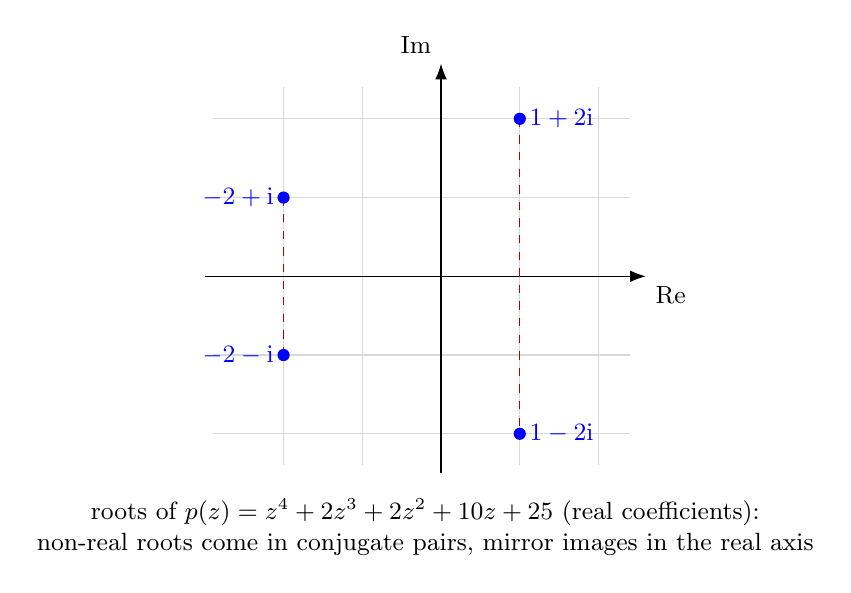
\begin{tikzpicture}[every node/.style={font=\small}, >={Latex[length=2mm]}]
	\draw[gray!30, step=1] (-2.9,-2.4) grid (2.4,2.4);
	\draw[->] (-3,0) -- (2.6,0) node[below right] {$\mathrm{Re}$};
	\draw[->] (0,-2.5) -- (0,2.7) node[above left] {$\mathrm{Im}$};
	\draw[dashed, red!70!black] (1,2) -- (1,-2);
	\draw[dashed, red!70!black] (-2,1) -- (-2,-1);
	\fill[blue] (1,2) circle (2.2pt) node[right] {$1+2\mathrm{i}$};
	\fill[blue] (1,-2) circle (2.2pt) node[right] {$1-2\mathrm{i}$};
	\fill[blue] (-2,1) circle (2.2pt) node[left] {$-2+\mathrm{i}$};
	\fill[blue] (-2,-1) circle (2.2pt) node[left] {$-2-\mathrm{i}$};
	\node[anchor=north, align=center] at (-0.2,-2.7) {roots of $p(z)=z^4+2z^3+2z^2+10z+25$ (real coefficients):\\ non-real roots come in conjugate pairs, mirror images in the real axis};
\end{tikzpicture}
\end{document}
